\documentclass[mathserif,serif]{beamer}
\usepackage{tabularx}
\setbeamertemplate{footline}[frame number]
% \useoutertheme{infolines}
\usepackage{slidesphysics}
\graphicspath{{../plot/}}

\title[]{Default/CFT comparison}
\author[]
{
Samuel Lo \inst{1}
\and
Yanjun Tu  \inst{1}
\and
Dongliang Zhang  \inst{2}
}
\institute[]
{
\inst{1}
The University of Hong Kong
\and
\inst{2}
University of Michigan
}
\date[]{\today}

\newcommand\Wider[2][3em]{%
\makebox[\linewidth][c]{%
\begin{minipage}{\dimexpr\textwidth+#1\relax}
\raggedright
\centering#2
\end{minipage}%
}%
}

\begin{document}
\frame{\titlepage}

\begin{frame}{Outline}
\tableofcontents
\end{frame}

\section{Introduction}
\begin{frame}{Introduction}
\begin{itemize}
\item Compare the event yield of the default and CFT setting.
\end{itemize}
\end{frame}

\section{SUSYTools config setting}
\begin{frame}{SUSYTools config setting}
Tool:
\begin{itemize}
\item AnalysisBase 2.4.31
\end{itemize}

SUSYTools Default setting:
\begin{itemize}
\item SUSYTools-00-08-60/data/SUSYTools\_Default.conf
\end{itemize}
CFT setting:
\begin{itemize}
\item Ele.Id: MediumLLH
\item Ele.Iso: FixedCutTight
\item Ele.CFT: Medium
\end{itemize}

Selection:
\begin{itemize}
\item Exactly 2 baseline leptons and exactly 2 signal leptons
\end{itemize}
\end{frame}

\section{Comparison of signal samples in SR}
\begin{frame}
\sectionpage
\end{frame}

\begin{frame}{Comparison of expected number of signal (175, 0)}
Use run 1 SR selection, see backup slides(page 17) for details.
\begin{tabular}{|c|c|c|}
\hline
Signal Region & Default & CFT \\
\hline
SR$ee$-1     & $7.1\pm1.2$ & $6.3\pm1.1$ \\
\hline
SR$ee$-2     & $2.0\pm0.5$ & $2.0\pm0.5$ \\
\hline
SR$\mu\mu$-1 & $5.4\pm0.8$ & $5.4\pm0.8$ \\
\hline
SR$\mu\mu$-2 & $10.1\pm1.4$ & $10.1\pm1.4$ \\
\hline
SR$e\mu$-1   & $8.0\pm1.1$ & $8.0\pm1.1$ \\
\hline
SR$e\mu$-2   & $4.9\pm0.7$ & $5.0\pm0.7$ \\
\hline
\end{tabular}
\end{frame}

\begin{frame}{Comparison of expected number of signal (165, 35)}
Use run 1 SR selection, see backup slides(page 17) for details.
\begin{tabular}{|c|c|c|}
\hline
Signal Region & Default & CFT \\
\hline
SR$ee$-1     & $2.4\pm0.4$ & $2.5\pm0.4$ \\
\hline
SR$ee$-2     & $0.9\pm0.2$ & $1.0\pm0.3$ \\
\hline
SR$\mu\mu$-1 & $2.5\pm0.5$ & $2.5\pm0.5$ \\
\hline
SR$\mu\mu$-2 & $4.2\pm0.5$ & $4.2\pm0.5$ \\
\hline
SR$e\mu$-1   & $5.3\pm0.6$ & $5.6\pm0.6$ \\
\hline
SR$e\mu$-2   & $2.5\pm0.4$ & $2.8\pm0.4$ \\
\hline
\end{tabular}
\end{frame}

\begin{frame}{Comparison of expected number of signal (400, 0)}
Use run 1 SR selection, see backup slides(page 17) for details.
\begin{tabular}{|c|c|c|}
\hline
Signal Region & Default & CFT \\
\hline
SR$ee$-1     & $9.8\pm0.8$ & $9.6\pm1.2$ \\
\hline
SR$ee$-2     & $4.3\pm0.6$ & $4.5\pm0.6$ \\
\hline
SR$\mu\mu$-1 & $8.7\pm0.8$ & $8.7\pm0.8$ \\
\hline
SR$\mu\mu$-2 & $7.7\pm0.7$ & $7.7\pm0.7$ \\
\hline
SR$e\mu$-1   & $14.7\pm1.1$ & $14.4\pm1.1$ \\
\hline
SR$e\mu$-2   & $9.2\pm0.8$ & $9.3\pm0.8$ \\
\hline
\end{tabular}
\end{frame}

\section{Comparison of Zee samples in SR}
\begin{frame}
\sectionpage
\end{frame}

\begin{frame}{Comparison of Zee samples in SR}
Use run 1 SR selection, see backup slides(page 17) for details.
\begin{tabular}{|c|c|c|}
\hline
Signal Region & Default & CFT \\
\hline
SR$ee$-1     & $10.9\pm15.8$ & $0.11\pm0.09$ \\
\hline
SR$ee$-2     & $1.9\pm2.0$ & $0.0\pm0.0$ \\
\hline
SR$\mu\mu$-1 & $0.0\pm0.0$ & $0.0\pm0.0$ \\
\hline
SR$\mu\mu$-2 & $0.0\pm0.0$ & $0.0\pm0.0$ \\
\hline
SR$e\mu$-1   & $0.0\pm0.0$ & $0.0\pm0.0$ \\
\hline
SR$e\mu$-2   & $0.05\pm0.05$ & $0.05\pm0.05$ \\
\hline
\end{tabular}
\end{frame}

\begin{frame}{Comparison of Zee samples in SRee-1}
The plot is without the mll cut. \\
The number is after the mll cut. \\
The CFT setting is used on the right plot for Zee and signal. \\
The default setting is used for VV and Vgamma for both plots. \\
The empty bin is due to a large negative weight of Zee.
\begin{columns}

\begin{column}{0.5\textwidth}
\begin{center}
\includegraphics[width=\textwidth]{mll_SR_SS_ee_1_def} \\
Default: Zee: $10.9\pm15.8$
\end{center}
\end{column}

\begin{column}{0.5\textwidth}
\begin{center}
\includegraphics[width=\textwidth]{mll_SR_SS_ee_1_cft} \\
CFT: Zee: $0.11\pm0.09$
\end{center}
\end{column}

\end{columns}

\end{frame}

\begin{frame}{Comparison of Zee samples in SRee-2}
\begin{columns}

\begin{column}{0.5\textwidth}
\begin{center}
\includegraphics[width=\textwidth]{mll_SR_SS_ee_2_def} \\
Default: Zee: $1.9\pm2.0$
\end{center}
\end{column}

\begin{column}{0.5\textwidth}
\begin{center}
\includegraphics[width=\textwidth]{mll_SR_SS_ee_2_cft} \\
CFT: Zee: $0.0\pm0.0$
\end{center}
\end{column}

\end{columns}

\end{frame}

\section{Comparison of Zee samples in CR}
\begin{frame}
\sectionpage
\end{frame}

\begin{frame}{Comparison of Zee samples in CR}
CR selection
\begin{itemize}
\item same-sign two leptons
\item $|m_{ll} - 91.2| < 10$
\end{itemize}
The plot is without the mll cut. \\
The number is after the mll cut. \\
The CFT setting is used on the right plot for Zee and signal. \\
The default setting is used for VV and Vgamma for both plots. \\

\begin{columns}

\begin{column}{0.5\textwidth}
\begin{center}
\includegraphics[width=\textwidth]{mll_CR_SS_ee_Zmass_def} \\
Default: Zee: $108,072\pm1,233$
\end{center}
\end{column}

\begin{column}{0.5\textwidth}
\begin{center}
\includegraphics[width=\textwidth]{mll_CR_SS_ee_Zmass_cft} \\
CFT: Zee: $17,207\pm572$
\end{center}
\end{column}

\end{columns}

\end{frame}

\section{Conclusion}
\begin{frame}{Conclusion}
\begin{itemize}
\item The Zee BG is reduced by 6 times, while the signal has small change.
\end{itemize}
\end{frame}

\begin{frame}
\begin{center}
\huge
Backup
\end{center}
\end{frame}

\begin{frame}{Selection}
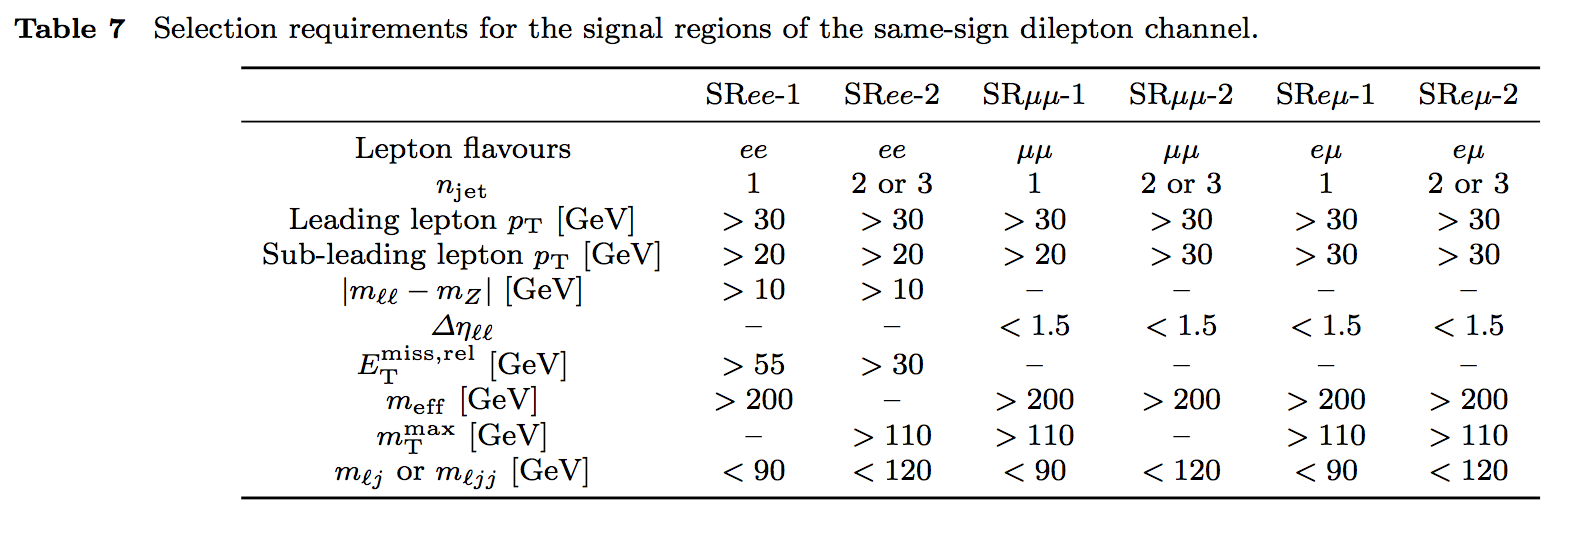
\includegraphics[width=\textwidth]{data/photo/SRcutrun1.png} \\
\url{https://arxiv.org/pdf/1501.07110.pdf}
\end{frame}

\begin{frame}[fragile]
\frametitle{Signal sample}
\small
Sample Name(p2972 tag):
\tiny
\begin{verbatim}
mc15_13TeV.993820.MGPy8EG_A14N13LO_C1N2_Wh_2L_175_0.merge.DAOD_SUSY2.e5678_a766_a821_r7676_p2949_p2972
mc15_13TeV.993821.MGPy8EG_A14N13LO_C1N2_Wh_2L_165_35.merge.DAOD_SUSY2.e5678_a766_a821_r7676_p2949_p2972
mc15_13TeV.993822.MGPy8EG_A14N13LO_C1N2_Wh_2L_400_0.merge.DAOD_SUSY2.e5678_a766_a821_r7676_p2949_p2972
\end{verbatim}
\end{frame}

\begin{frame}[fragile]
\frametitle{Background Z+jets(Sherpa)}
\small
Sample Name(p2879 tag):
\tiny
\begin{verbatim}
364114.Sherpa_221_NNPDF30NNLO_Zee_MAXHTPTV0_70_CVetoBVeto.merge.DAOD_SUSY2.e5299_s2726_r7772_r7676_p2879
364115.Sherpa_221_NNPDF30NNLO_Zee_MAXHTPTV0_70_CFilterBVeto.merge.DAOD_SUSY2.e5299_s2726_r7772_r7676_p2879
364116.Sherpa_221_NNPDF30NNLO_Zee_MAXHTPTV0_70_BFilter.merge.DAOD_SUSY2.e5299_s2726_r7772_r7676_p2879
364117.Sherpa_221_NNPDF30NNLO_Zee_MAXHTPTV70_140_CVetoBVeto.merge.DAOD_SUSY2.e5299_s2726_r7772_r7676_p2879
364118.Sherpa_221_NNPDF30NNLO_Zee_MAXHTPTV70_140_CFilterBVeto.merge.DAOD_SUSY2.e5299_s2726_r7772_r7676_p2879
364119.Sherpa_221_NNPDF30NNLO_Zee_MAXHTPTV70_140_BFilter.merge.DAOD_SUSY2.e5299_s2726_r7772_r7676_p2879
364120.Sherpa_221_NNPDF30NNLO_Zee_MAXHTPTV140_280_CVetoBVeto.merge.DAOD_SUSY2.e5299_s2726_r7772_r7676_p2879
364121.Sherpa_221_NNPDF30NNLO_Zee_MAXHTPTV140_280_CFilterBVeto.merge.DAOD_SUSY2.e5299_s2726_r7772_r7676_p2879
364122.Sherpa_221_NNPDF30NNLO_Zee_MAXHTPTV140_280_BFilter.merge.DAOD_SUSY2.e5299_s2726_r7772_r7676_p2879
364123.Sherpa_221_NNPDF30NNLO_Zee_MAXHTPTV280_500_CVetoBVeto.merge.DAOD_SUSY2.e5299_s2726_r7772_r7676_p2879
364124.Sherpa_221_NNPDF30NNLO_Zee_MAXHTPTV280_500_CFilterBVeto.merge.DAOD_SUSY2.e5299_s2726_r7772_r7676_p2879
364125.Sherpa_221_NNPDF30NNLO_Zee_MAXHTPTV280_500_BFilter.merge.DAOD_SUSY2.e5299_s2726_r7772_r7676_p2879
364126.Sherpa_221_NNPDF30NNLO_Zee_MAXHTPTV500_1000.merge.DAOD_SUSY2.e5299_s2726_r7772_r7676_p2879
364127.Sherpa_221_NNPDF30NNLO_Zee_MAXHTPTV1000_E_CMS.merge.DAOD_SUSY2.e5299_s2726_r7772_r7676_p2879
\end{verbatim}
\end{frame}

\begin{frame}[fragile]
\frametitle{Background Di-Boson(Sherpa)}
\small
Sample Name(p2879 tag):
\tiny
\begin{verbatim}
mc15_13TeV.363490.Sherpa_221_NNPDF30NNLO_llll.merge.DAOD_SUSY2.e5332_s2726_r7772_r7676_p2879
mc15_13TeV.363491.Sherpa_221_NNPDF30NNLO_lllv.merge.DAOD_SUSY2.e5332_s2726_r7772_r7676_p2879
mc15_13TeV.363492.Sherpa_221_NNPDF30NNLO_llvv.merge.DAOD_SUSY2.e5332_s2726_r7772_r7676_p2879
mc15_13TeV.361069.Sherpa_CT10_llvvjj_ss_EW4.merge.DAOD_SUSY2.e3836_s2726_r7772_r7676_p2879
mc15_13TeV.361070.Sherpa_CT10_llvvjj_ss_EW6.merge.DAOD_SUSY2.e3836_s2608_r7772_r7676_p2879
mc15_13TeV.361071.Sherpa_CT10_lllvjj_EW6.merge.DAOD_SUSY2.e3836_s2608_s2183_r7772_r7676_p2879
mc15_13TeV.361072.Sherpa_CT10_lllljj_EW6.merge.DAOD_SUSY2.e3836_s2608_s2183_r7772_r7676_p2879
mc15_13TeV.361073.Sherpa_CT10_ggllll.merge.DAOD_SUSY2.e3836_s2608_s2183_r7772_r7676_p2879
mc15_13TeV.361077.Sherpa_CT10_ggllvv.merge.DAOD_SUSY2.e3836_s2608_s2183_r7772_r7676_p2879
mc15_13TeV.363358.Sherpa_221_NNPDF30NNLO_WqqZll.merge.DAOD_SUSY2.e5525_s2726_r7772_r7676_p2879
mc15_13TeV.363356.Sherpa_221_NNPDF30NNLO_ZqqZll.merge.DAOD_SUSY2.e5525_s2726_r7772_r7676_p2879
\end{verbatim}
\end{frame}

\begin{frame}[fragile]
\frametitle{Background V+gamma(Sherpa)}
\small
Sample Name(p2879 tag):
\tiny
\begin{verbatim}
mc15_13TeV.301535.Sherpa_CT10_eegammaPt10_35.merge.DAOD_SUSY2.e3952_s2608_s2183_r7725_r7676_p2879
mc15_13TeV.301536.Sherpa_CT10_mumugammaPt10_35.merge.DAOD_SUSY2.e3952_s2608_s2183_r7725_r7676_p2879
mc15_13TeV.301890.Sherpa_CT10_enugammaPt35_70.merge.DAOD_SUSY2.e3952_s2608_s2183_r7725_r7676_p2879
mc15_13TeV.301891.Sherpa_CT10_enugammaPt70_140.merge.DAOD_SUSY2.e3952_s2608_s2183_r7725_r7676_p2879
mc15_13TeV.301892.Sherpa_CT10_enugammaPt140.merge.DAOD_SUSY2.e3952_s2608_s2183_r7725_r7676_p2879
mc15_13TeV.301893.Sherpa_CT10_munugammaPt35_70.merge.DAOD_SUSY2.e3952_s2608_s2183_r7725_r7676_p2879
mc15_13TeV.301894.Sherpa_CT10_munugammaPt70_140.merge.DAOD_SUSY2.e3952_s2608_s2183_r7725_r7676_p2879
mc15_13TeV.301895.Sherpa_CT10_munugammaPt140.merge.DAOD_SUSY2.e3952_s2608_s2183_r7725_r7676_p2879
mc15_13TeV.301896.Sherpa_CT10_taunugammaPt35_70.merge.DAOD_SUSY2.e3952_s2608_s2183_r7725_r7676_p2879
mc15_13TeV.301897.Sherpa_CT10_taunugammaPt70_140.merge.DAOD_SUSY2.e3952_s2608_s2183_r7725_r7676_p2879
mc15_13TeV.301898.Sherpa_CT10_taunugammaPt140.merge.DAOD_SUSY2.e3952_s2608_s2183_r7725_r7676_p2879
mc15_13TeV.301899.Sherpa_CT10_eegammaPt35_70.merge.DAOD_SUSY2.e3952_s2608_s2183_r7725_r7676_p2879
mc15_13TeV.301900.Sherpa_CT10_eegammaPt70_140.merge.DAOD_SUSY2.e3952_s2608_s2183_r7725_r7676_p2879
mc15_13TeV.301901.Sherpa_CT10_eegammaPt140.merge.DAOD_SUSY2.e3952_s2608_s2183_r7725_r7676_p2879
mc15_13TeV.301902.Sherpa_CT10_mumugammaPt35_70.merge.DAOD_SUSY2.e3952_s2608_s2183_r7725_r7676_p2879
mc15_13TeV.301903.Sherpa_CT10_mumugammaPt70_140.merge.DAOD_SUSY2.e3952_s2608_s2183_r7725_r7676_p2879
mc15_13TeV.301904.Sherpa_CT10_mumugammaPt140.merge.DAOD_SUSY2.e3952_s2608_s2183_r7725_r7676_p2879
mc15_13TeV.301905.Sherpa_CT10_tautaugammaPt35_70.merge.DAOD_SUSY2.e3952_s2608_s2183_r7725_r7676_p2879
mc15_13TeV.301906.Sherpa_CT10_tautaugammaPt70_140.merge.DAOD_SUSY2.e3952_s2608_s2183_r7725_r7676_p2879
mc15_13TeV.301907.Sherpa_CT10_tautaugammaPt140.merge.DAOD_SUSY2.e3952_s2608_s2183_r7725_r7676_p2879
\end{verbatim}
\end{frame}

\end{document}
